\chapter{Anhang}
\label{cha:anh}

\captionsetup{list=false}

\section*{Klassendiagramm}
\label{sec:anh:class}

\begin{figure}[H]
\centering
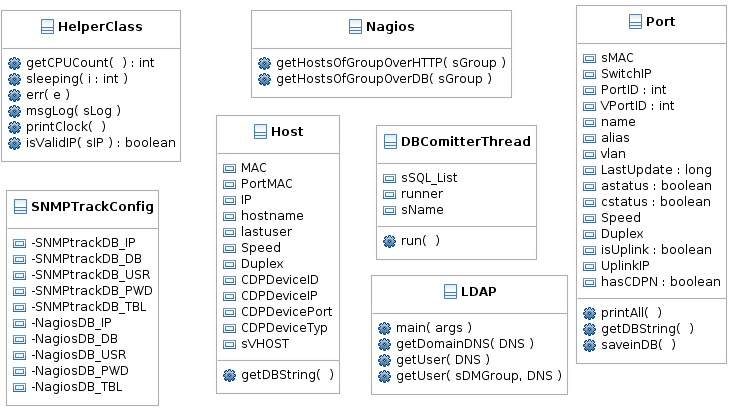
\includegraphics[width=1.0\textwidth]{model1.png}
\caption[]{Klassendiagramm}
\label{fig:classdia1}
\end{figure}

\begin{figure}[H]
\centering
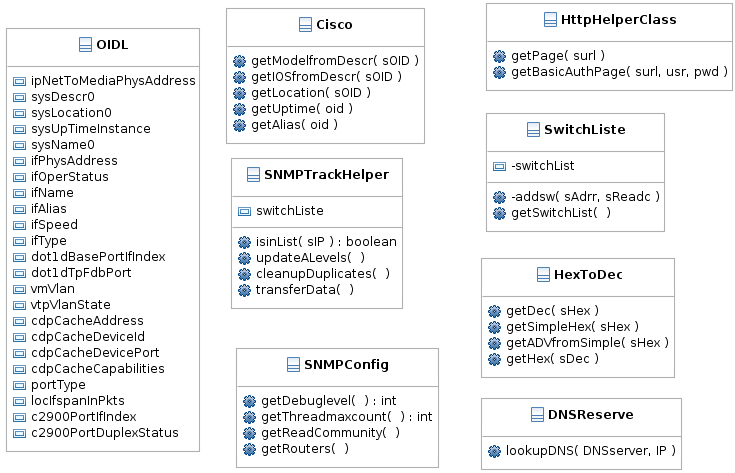
\includegraphics[width=1.0\textwidth]{model2.png}
\caption[]{Klassendiagramm}
\label{fig:classdia2}
\end{figure}

\begin{figure}[H]
\centering
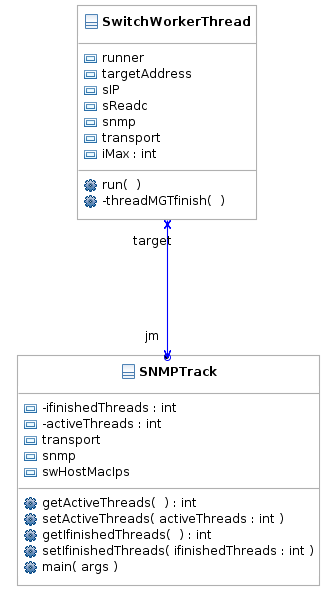
\includegraphics[width=0.4\textwidth]{model3.png}
\caption[]{Klassendiagramm}
\label{fig:classdia3}
\end{figure}

\begin{figure}[H]
\centering
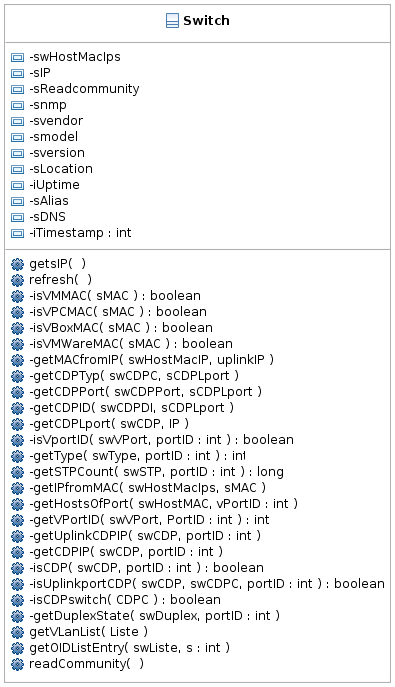
\includegraphics[width=0.6\textwidth]{model4.png}
\caption[]{Klassendiagramm}
\label{fig:classdia4}
\end{figure}

\begin{figure}[H]
\centering
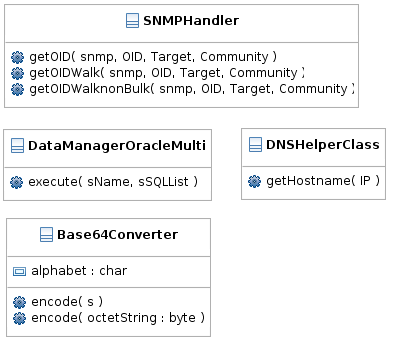
\includegraphics[width=0.6\textwidth]{model5.png}
\caption[]{Klassendiagramm}
\label{fig:classdia5}
\end{figure}

\begin{figure}[H]
\centering
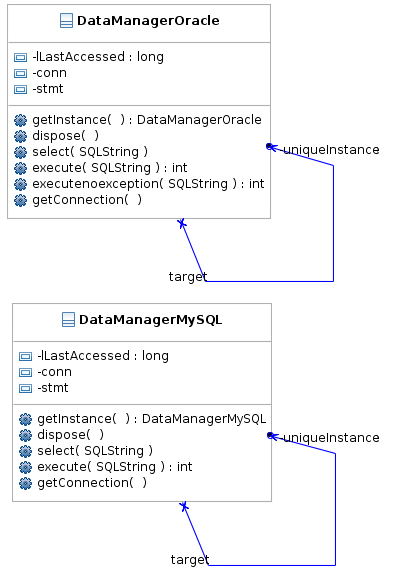
\includegraphics[width=0.6\textwidth]{model6.png}
\caption[]{Klassendiagramm}
\label{fig:classdia6}
\end{figure}

\section*{Konfiguration SNMP-Track}
\label{sec:config}

\begin{figure}[H]
\centering
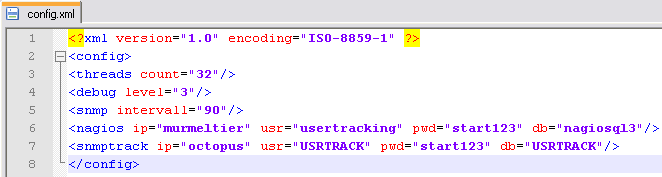
\includegraphics[width=1.0\textwidth]{config_xml.png}
\caption[]{config.xml}
\label{fig:config_xml}
\end{figure}


\section*{Benchmarkwerte}
\label{sec:Anhang2}

Noch leer.